\section{岭回归}
\subsection{自己实现的岭回归与自带包实现的岭回归}
选取超参数$\lambda$为$0.01$,使用两种不同的代码实现岭回归,得到模型中的参数如下表所示

\begin{table}[htbp]
\centering
\begin{tabular}{ccccccccccccccc}
  \hline
 & 截距项 & crim & zn & indus & chas & nox & rm & age & dis & rad & tax & ptratio & black & lstat \\ 
  \hline
  手写代码 & 35.96 & -0.11 & 0.05 & 0.02 & 2.69 & -17.48 & 3.83 & 0.00 & -1.47 & 0.30 & -0.01 & -0.95 & 0.01 & -0.52 \\ 
  自带包& 36.46 & -0.11 &  0.05 &  0.02  & 2.69 &-17.76 &3.81  & 0.00&  -1.48&   0.31 & -0.01&  -0.95&0.01&-0.52\\
   \hline
\end{tabular}
\end{table}

\subsection{基于交叉验证选择最佳参数}

自动选择参数$\lambda$值的范围进行岭回归,选择在 $\lambda =1$到 $\lambda = 10^{-3}$的范围内进行岭回归,如图所示可得每个变量的系数随着参数$\lambda$变化所得到的曲线.
\begin{figure}[htbp]
  \centering
  \caption{系数变化曲线}
  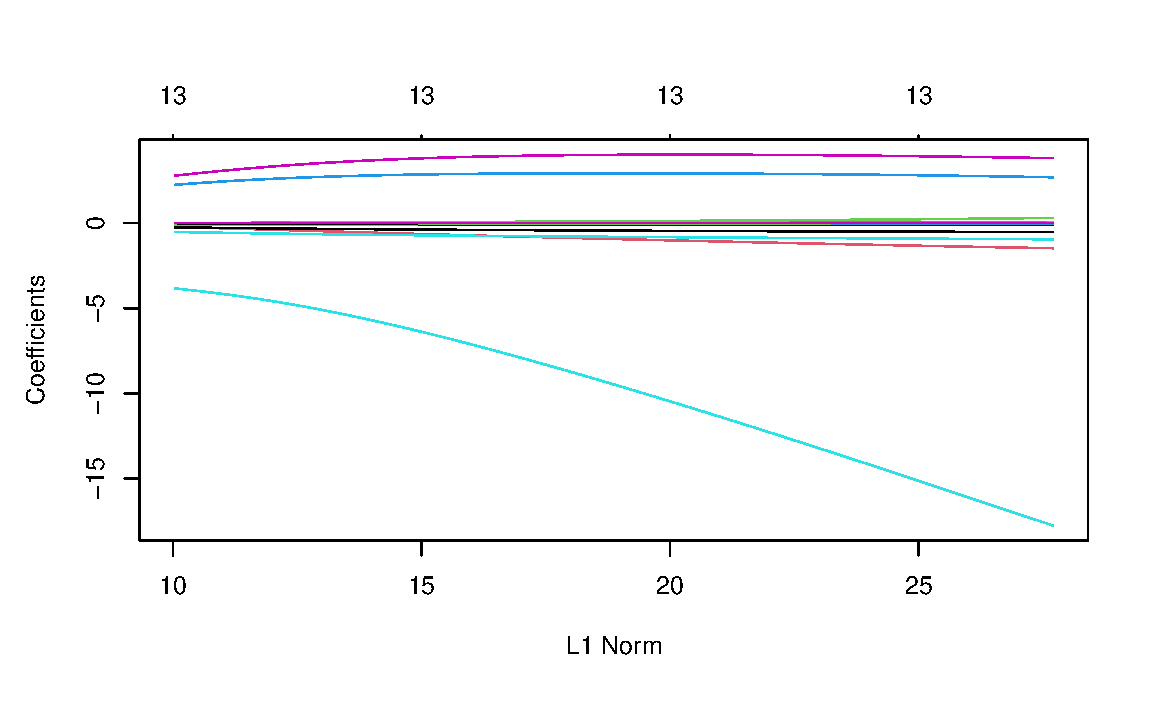
\includegraphics[width=0.8\textwidth]{opt_para.eps}
\end{figure}

将数据分为10折,使用交叉验证法选择调节参数$\lambda$,得到系数变化曲线如下图所示
\begin{figure}[htbp]
  \centering
  \caption{交叉验证法的系数变化曲线}
  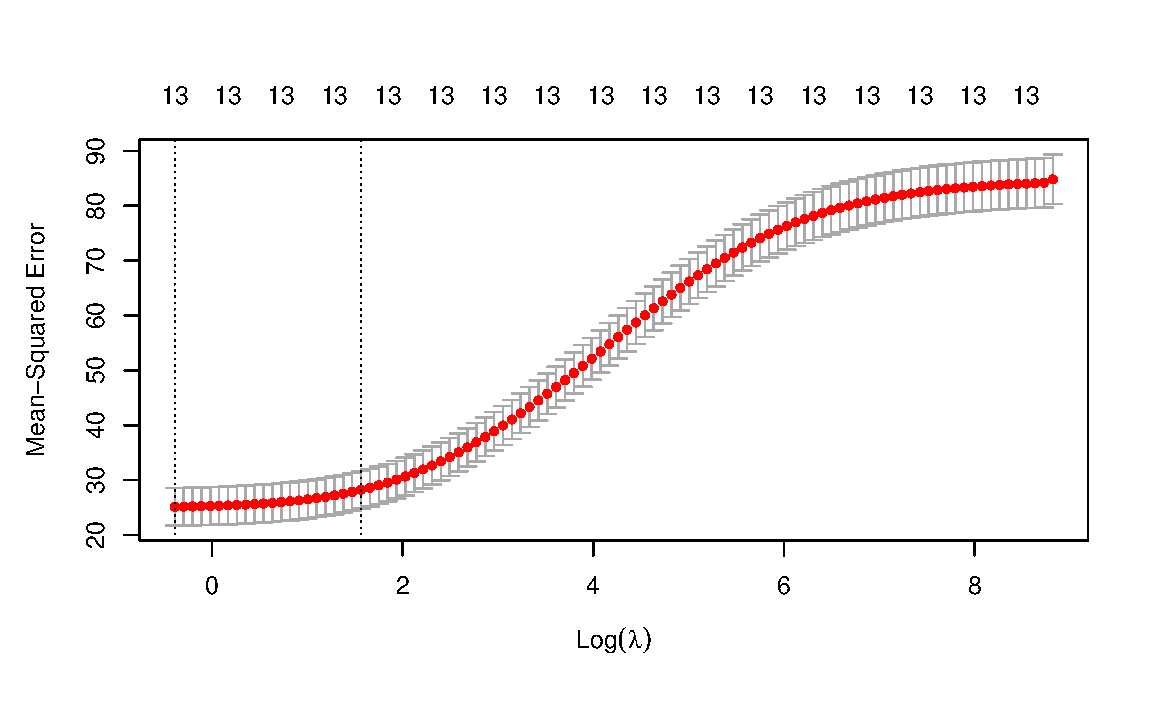
\includegraphics[width=0.6\textwidth]{cv_para.eps}
\end{figure}

分别选取$\lambda$的LSE值以及最小的$\lambda$值下的变量系数,如下图所示
\begin{figure}[htbp]
  \centering
  \caption{两个$\lambda$值下的系数}
  \includegraphics[width=0.6\textwidth]{coef.jpg}
\end{figure}
